\documentclass{abntex2}
\usepackage[utf8]{inputenc}
\usepackage{graphicx}
\usepackage[num]{abntex2cite}



\titulo{Experimento 4: Caracterização e ganho de emissor comum}
\autor{Lucas Rezende de Macedo - 14/0026363\\Jônatas Ribeiro Senna Pires - 14/0090983}
\data{12 de Maio de 2018}
\local{Brasília, Distrito Federal}

\begin{document}

\imprimircapa
\imprimirfolhaderosto

\tableofcontents
\listoffigures
\clearpage

\chapter{Experiências}

 O objetivo das experiências realizadas consiste na caracterização de transistores NPN
 por meio do circuito descrito na figura
 \ref{fig:circuito}

\begin{figure}[h]
  \centering
  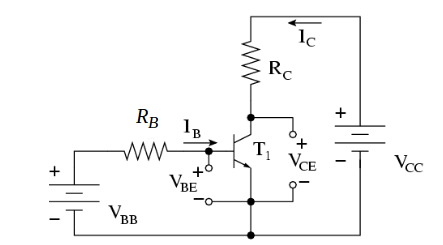
\includegraphics[scale = 0.5]{circuito.png}
  \caption{Circuito de caracterização de transistores NPN.}
  \label{fig:circuito}
\end{figure}


\section{Experiência}
\subsection{Experiência 1}

Foi montado o circuito da figura \ref{fig:circuito} com os seguintes parâmetros:
\begin{itemize}
  \item $R_B = 9,86K\Omega $
  \item $R_C = 99,62\Omega$
  \item $T_1 = BC548$
\end{itemize}

Ajustando a fonte de tensão para que $V_B_B$ assuma os valores -2V, -1V, 0V, 0.5V, 1V, 2V, 3V e 5V
, foi medido $V_B_E$ e $V_C_E$ e a partir dos valores coletados, foram calculados os valores de $I_B$ e $I_C$ de acordo com as seguintes expressões:
\begin{itemize}
  \item $I_B = (V_B_B - V_B_E) / R_B$
  \item $I_C = (V_C_C - V_C_E) / R_C$
\end{itemize}

Após o cálculo do valor das correntes, foi construída uma tabela para cada valor de $V_C_C$ pedido
(10V, 5V e 0V), respectivamente, neste relatório, a tabela \ref{tab:exp11}, a tabela \ref{tab:exp12} e a tabela \ref{tab:exp13}.

\begin{table}[h]
\centering
\begin{tabular}{|l|l|l|l|l|}
\hline
$V_{BB}(V)$ & $V_{BE}$(V) & $V_{CE}$(V) & $I_B$ (A) & $I_C$ (A) \\
\hline
-2        & -2      & 9,97                              & 0             & 0,30m                  \\
\hline
-1         & -1      &  9,97                          & 0             & 0,30m                  \\
\hline
0           & 4,35m      & 9,99                           & -43,98             & 0,10m                  \\
\hline
0,5        & 0,5      & 9,98                           & 0             & 0,20m                  \\
\hline
1         & 0,62      & 8,65                           & 384,22m             & 13,55m                  \\
\hline
2         & 0,65      & 5,58                           & 0,13m             & 44,36m                  \\
\hline
3         & 0,7      & 3,43                          & 0,23m             & 65,95m                  \\
\hline
5         & 0,767      & 2,18                           & 0,42m             & 78,49m                  \\
\hline
\end{tabular}
\label{tab:exp11}
\caption{Tabela com os valores de $V_{BB}$, $V_{BE}$, $V_{CE}$, $I_B$, $I_C$ para $V_{CC} = 10V$.}
\end{table}

\begin{table}[h]
\centering
\begin{tabular}{|l|l|l|l|l|}
\hline
$V_{BB}(V)$ & $V_{BE}$(V) & $V_{CE}$(V) & $I_B$ (A) & $I_C$ (A) \\
\hline
-2        & -2      & 4,99                              & 0             & 0,10m                  \\
\hline
-1         & -1      &  4,99                          & 0             & 0,10m                  \\
\hline
0           & 4,4m      & 4,99                           & -44,48\mu             & 0,10m                  \\
\hline
0.5        & 0,5      & 4,98                           & 0             & 0,20m                  \\
\hline
1         & 0,68      & 4,05                           & 323,55m             & 9,53m                  \\
\hline
2        & 0,83      & 1,59                           & 0,11m             & 34,23m                  \\
\hline
3         & 0,87      & 0,75                           & 0,21m             & 42,66m                  \\
\hline
5         & 0,78      & 0,29                           & 0,42m             & 47,27m                  \\
\hline
\end{tabular}
\label{tab:exp12}
\caption{Tabela com os valores de $V_{BB}$, $V_{BE}$, $V_{CE}$, $I_B$, $I_C$ para $V_{CC} = 5V$.}
\end{table}

\begin{table}[h]
\centering
\begin{tabular}{|l|l|l|l|l|}
\hline
$V_{BB}(V)$ & $V_{BE}$(V) & $V_{CE}$(V) & $I_B$ (A) & $I_C$ (A) \\
\hline
-2        & -2      & 0                              & 0             & 0                  \\
\hline
-1         & -1      &  0                          & 0             & 0                  \\
\hline
0           & 4,44m      & 0                           & -44,89\mu             & 0                  \\
\hline
0,5        & 0,48      & 0                           & 2,02\mu            & 0                  \\
\hline
1         & 0,58      & 2,30m                           & 424,67m             & -230,87m                  \\
\hline
2         & 0,63      & 3,83m                           & 0,13m             & -384,46m                  \\
\hline
3         & 0,65      & 5,00m                          & 0,23m             & -501,90m                  \\
\hline
5         & 0,676      & 4,28m                           & 0,43m             & -429,63m                  \\
\hline
\end{tabular}
\label{tab:exp13}
\caption{Tabela com os valores de $V_{BB}$, $V_{BE}$, $V_{CE}$, $I_B$, $I_C$ para $V_{CC} = 0V$.}
\end{table}

\subsection{Experiência 2}

Foi montado o circuito da figura \ref{fig:circuito} com os seguintes parâmetros:
\begin{itemize}
  \item $R_B = 9,86K\Omega $
  \item $R_C = 298,8\Omega$
\end{itemize}

Para esta parte do experimento foram utilizados dois transistores NPN BC548 distintos para aferição dos valores.
\\Ajustando a fonte de tensão $V_B_B$ de forma que $V_C_E$ assuma o valor de 5V.
Foi medido $V_B_E$, $V_C_E$ e $V_B_B$ e a partir dos valores coletados, foram calculados os valores de $I_B$ e $I_C$ de acordo com as seguintes expressões:
\begin{itemize}
  \item $I_B = (V_B_B - V_B_E) / R_B$
  \item $I_C = (V_C_C - V_C_E) / R_C$
\end{itemize}
Após o cálculo do valor das correntes, foi construída a tabela \ref{tab:exp21} com os valores obtidos.

Nesta parte da experiência, mantendo os parâmetros para $R_B$ e $R_C$, foram utilizados dois transistores NPN TIP31 distintos para aferição dos valores.
\\Ajustando a fonte de tensão $V_B_B$ de forma que $V_C_E$ assuma o valor de 5V.
Foi medido $V_B_E$, $V_C_E$ e $V_B_B$ e a partir dos valores coletados, foram calculados os valores de $I_B$ e $I_C$ de acordo com as seguintes expressões:
\begin{itemize}
  \item $I_B = (V_B_B - V_B_E) / R_B$
  \item $I_C = (V_C_C - V_C_E) / R_C$
\end{itemize}
Após o cálculo do valor das correntes, foi construída a tabela \ref{tab:exp22} com os valores obtidos.

\begin{table}[h]
\centering
\begin{tabular}{|l|l|l|l|l|l|l|l|l|}
\hline
  & $V_{CC}$ (V) & $V_{CE}$ (V) & $V_{BB}$ (V) & $V_{BE}$ (V) & $R_B$ (\Omega) & $R_C$ (\Omega) & $I_C$ (A) & $I_B$ (A) \\
\hline
T1  & 10 & 5 & 1,2 & 0,68 & 9,89k & 298,8 & 16,73m & 525,78m \\
\hline
T2  & 10 & 5 & 1,21 & 0,69 & 9,89k & 298,8 & 16,73m & 525,78m \\
\hline
\end{tabular}
\label{tab:exp21}
\caption{Tabela com os valores de $V_{CC}$ $V_{CE}$, $V_{BB}$, $V_{BE}$, $R_B$, $R_C$, $I_B$, $I_C$ para os transistores BC548.}
\end{table}

\begin{table}[h]
\centering
\begin{tabular}{|l|l|l|l|l|l|l|l|l|}
\hline
  & $V_{CC}$ (V) & $V_{CE}$ (V) & $V_{BB}$ (V) & $V_{BE}$ (V) & $R_B$ (\Omega) & $R_C$ (\Omega) & $I_C$ (A) & $I_B$ (A) \\
\hline
T1  & 10 & 5 & 3,09 & 0,67 & 9,89k & 298,8 & 16,73m & 0,24m \\
\hline
T2  & 10 & 5 & 3,00 & 0,70 & 9,89k & 298,8 & 16,73m & 0,23m \\
\hline
\end{tabular}
\label{tab:exp22}
\caption{Tabela com os valores de $V_{CC}$ $V_{CE}$, $V_{BB}$, $V_{BE}$, $R_B$, $R_C$, $I_B$, $I_C$ para os transistores TIP31.}
\end{table}

\chapter{Discussão}

\section{Questão 1 - Construção dos gráficos}


\section{Questão 2 - Estimar \Beta}



\section*{Referências}


[1] SEDRA, Adel S.; SMITH, Kenneth Carless. Microelectronic circuits. New York: Oxford University Press, 1998.

[2] RAZAVI, Behzad; BEHZAD, Razavi. RF microelectronics. New Jersey: Prentice Hall, 1998.

[3] MIRZAEE, Mohammad Reza, et. al. “Simulating of human cardiovascular system and blood vessel
obstruction using lumped method”. World Academy of Science, Engineering and Technology, 2008, vol.
41.

[4] MOSSA, Hassanain Ali Lafta Mossa. “Engineering Modeling of Human Cardiovascular System”. 1st
International Conference of Eng. Sci. NUCEJ Spatial ISSUE, vol. 11, no. 2, Proceedings, 2008. pp. 307-
314.

[5] O CORAÇÃO COMO BOMBA (HIDRÁULICA). ROCHA,  Adson. Disponível em: $https://youtu.be/yhnFyU_M-uQ$. Acesso em: 14 abr. 2018.

\end{document}
